\section{Pipeline}

Surface Reconstruction from Point Sets is a sequential process:

\begin{itemize}
\item Scanning and scan alignment produce a set of points
      or points with normals. Alignment is not yet
      covered by \cgal.
\item Outlier removal for reconstruction methods which
      are not resilient to outliers.
\item Simplification to reduce the number of input points.
\item Smoothing to reduce noise in the input data.
\item Normal estimation and orientation when the normals
      are not already provided by the acquisition device.
\item Surface reconstruction.
\end{itemize}

\cgal\ provides algorithms for all steps listed above except alignment.\\
Chapter \ccc{Point_set_processing_3} \ref{chap:point_set_processing_3} describes outlier removal, simplification, smoothing,
normal estimation and orientation.\\
This package provides surface reconstruction using \cgal\ Surface Mesh Generator.

% Insert image pipeline.jpg/eps
\begin{center}
    \label{Surface_reconstruction_points_3-fig-pipeline}
    % Image
    \begin{ccTexOnly}
        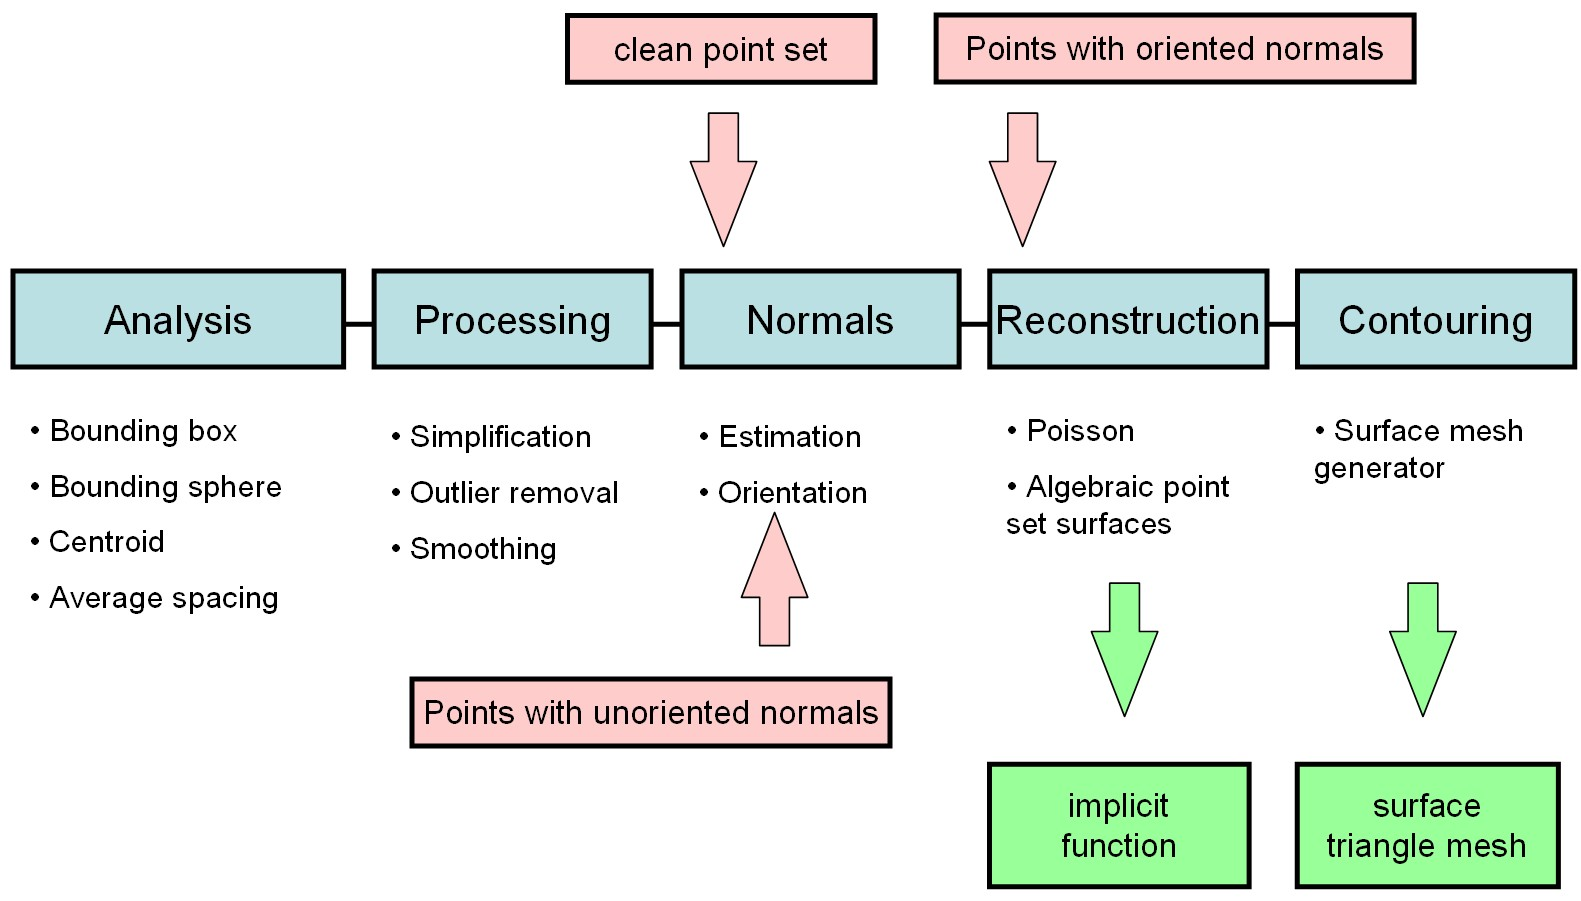
\includegraphics[width=1.0\textwidth]{Surface_reconstruction_points_3/pipeline} % omit .eps suffix
    \end{ccTexOnly}
    \begin{ccHtmlOnly}
        <img width="70%" border=0 src="./pipeline.jpg"><P>
    \end{ccHtmlOnly}
    % Title
    \begin{figure}[h]
        \caption{Surface Reconstruction from Point Sets pipeline.}
    \end{figure}
\end{center}



